\documentclass{article}

\usepackage{caption}

\usepackage{multirow}

\usepackage{graphicx}
\setlength{\abovecaptionskip}{10pt plus 3pt minus 2pt}
\setlength{\belowcaptionskip}{10pt plus 3pt minus 2pt}

\usepackage[margin=1in]{geometry}

\usepackage{algorithm,algpseudocode}

\usepackage{xcolor}
\usepackage{listings}
\lstdefinestyle{DOS}{
    backgroundcolor=\color{lightgray},
    basicstyle=\scriptsize\color{black}\ttfamily
}

\usepackage{hyperref}
\hypersetup{
    pdfborderstyle={/S/U/W 1},
    colorlinks=true,
    linkcolor=blue,
    filecolor=magenta,
    urlcolor=cyan,
}

\title{\vspace{-4em}
CSE 5441 (Fall 2019, Dr. Jones)\\
\large \texttt{MPI} + Hierarchical Parallelism (Lab 5)
}
\author{
Caleb Lehman \\
\href{mailto:lehman.346@osu.edu}{lehman.346@osu.edu}
}
\date{}

\begin{document}
\maketitle

\section*{Overview}
\label{sec:overview}

For this lab, I parallelized my serial \texttt{C} program to perform Adaptive
Mesh Refinement (AMR)\footnote{See lab 1 or project descriptions for details
about AMR computation.} using \texttt{MPI} and \texttt{OpenMP}. In particular,
the program launches 5 MPI ranks, 4 of which execute computations in parallel,
which utilizes the inter-node parallelism available in a large cluster. Within
each of the 4 computational ranks, I used \texttt{OpenMP} to exploit intra-node
parallelism. I found that I was able to get some additional speed-up from the
\texttt{OpenMP} threads, but it did not scale to using all of the available cores
on the nodes. Full results are in the results section.

\section*{Tests}
\label{sec:tests}

\subsection*{Environment}
\label{subsec:environment}

The program was developed and tested on the
\href{https://www.osc.edu/resources/technical_support/supercomputers/pitzer}{Pitzer
cluster} at the \href{https://www.osc.edu/}{Ohio Supercomputer Center}. Note that
the original assigment specified that we should use the
\href{https://www.osc.edu/resources/technical_support/supercomputers/owens}{Owens
cluster}, however, my first 3 labs were developed and tested on Pitzer, and after
bringing this up with Dr. Jones, he permitted me to perform this lab on Pitzer,
for comparison's sake.

For development and testing, I loaded the \texttt{mvapich2/2.3} and \texttt{intel/18.0.3} modules, which
allowed the program to be compiled with the \texttt{mpicc} compiler, using version 18.0.3 of the \texttt{icc}
compiler a the default \texttt{C} compiler, as well as setting some environment variables pointing to
\texttt{MPI}-related headers and libraries.

For testing, I loaded the \texttt{python/3.6-conda5.2} module, which loads a
python environment with the \texttt{NumPy}, \texttt{SciPy}, and
\texttt{Matplotlib} packages, amoung others. \texttt{Python} is only necessary
for collecting and plotting the data from testing, not for the actual exectuion
of the program.

\subsection*{Timing}
\label{subsec:timing}

I collected timing data using the same 4 methods as the first several labs:
\texttt{time}, \texttt{clock}, and \texttt{clock\textunderscore gettime} from
the \texttt{"time.h"} header, and the \texttt{UNIX} utility \texttt{time}.

As with the second and third labs, I didn't use the results from the \texttt{clock}
function from the \texttt{"time.h"} header, since it reports CPU time, not wall
time. In this case, that would have been fine, since the rank 0 \texttt{MPI} process
doesn't spawn any other threads, but to be consistent with previous labs,
\emph{I used the \texttt{clock\textunderscore gettime}
function for all results in this report}.

\subsection*{Test Files}
\label{subsec:test_files}

Dr. Jones provided the \texttt{testgrid\textunderscore 400\textunderscore
12206} test file.  As part of lab 1, I reduced the $\alpha$ (affect rate) and
$\varepsilon$ parameters until the serial runtime increased into the 3 to 6
minute range. In particular, I selected $\alpha = 0.01$ and $\varepsilon =
0.02$, for which the serial program completed in 261 seconds.

The above approach of changing the $\alpha$ and $\epsilon$ parameters allows us
to make the programs run longer, but doesn't affect the actual length of each
iteration. With only 12206 boxes, each iteration is fairly short (on the order
of $\frac{261\textrm{ sec}}{1589637} = 0.16\textrm{ms}$ per iteration), so I
expected the overhead of synchronizing processes and threads would inhibit parallelizing
beyond a small number of processes and threads. In order to investigate this, I generated
another test file, \texttt{testgrid\textunderscore 1000\textunderscore 296793},
which has more boxes and therefore longer iterations. I used values of
$(\alpha=0.9, \varepsilon=0.9)$ for this test case, since they produced a
serial runtime of around 3 minutes. I used this test case for each of labs 2 and 3,
so I also tested with it in this lab.

\begin{table}[H]
    \centering
    \begin{tabular}{|c|c|c|c|c|c|}
        \hline
        test & \texttt{\#} rows & \texttt{\#} cols & \texttt{\#} boxes & mean \texttt{\#} neighbors & std. dev. \texttt{\#} neighbors \\
        \hline
        \hline
        \texttt{testgrid\textunderscore 400\textunderscore 12206} & 400 & 400 & 12206 & 5.89 & 1.55 \\
        \texttt{testgrid\textunderscore 1000\textunderscore 296793} & 1000 & 1000 & 296793 & 4.79 & 1.57 \\
        \hline
    \end{tabular}
    
    \caption{Basic statistics for the test files.}

\end{table}

\section*{Results}
\label{sec:results}

The output for both test cases was as follows:

\begin{itemize}
    \item \texttt{testgrid\textunderscore 400\textunderscore 12206}: 1589637 iterations, $(max, min) = (0.085900, 0.084182)$
    \item \texttt{testgrid\textunderscore 1000\textunderscore 296793}: 51684 iterations, $(max, min) = (0.000000, 0.000000)$
\end{itemize}

I obtained the following timing results (current lab results in Figure 1, overall course results in Table 2):

\begin{figure}[H]
    \centering
    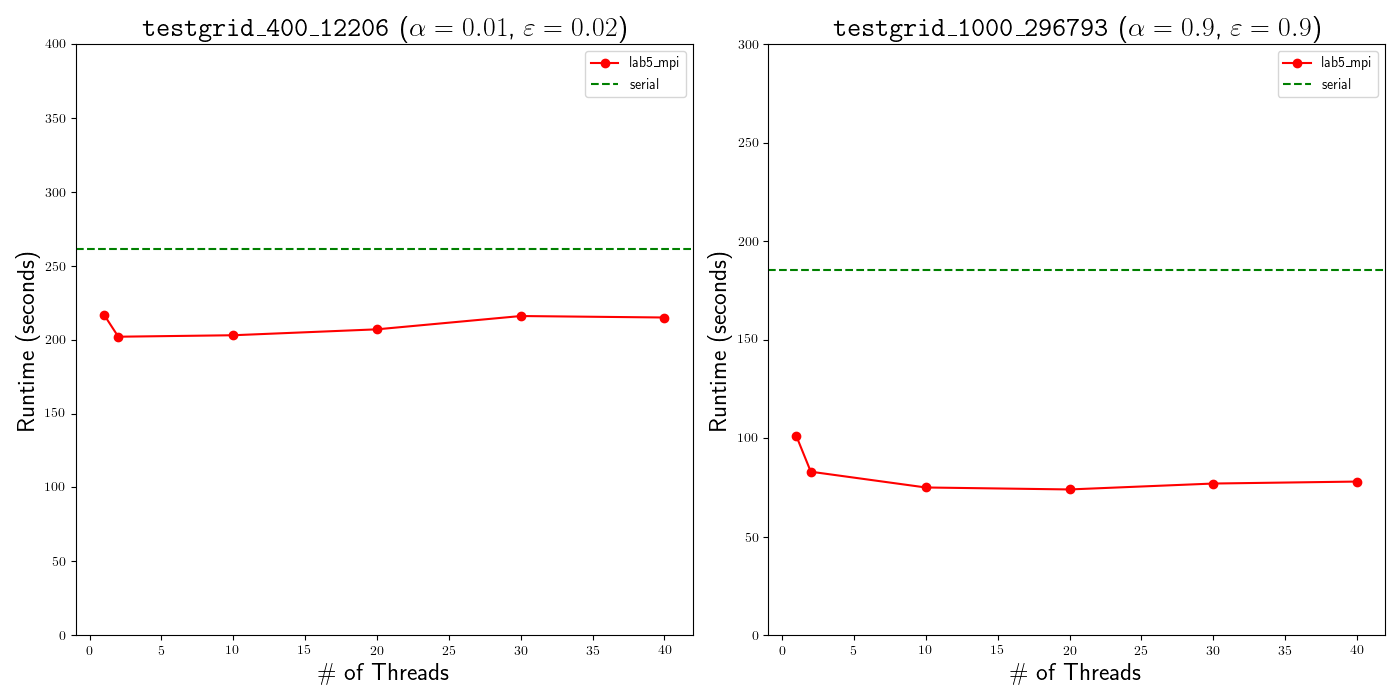
\includegraphics[width=.8\linewidth]{../plot.png}
    \caption{Runtimes for various numbers of threads. The \texttt{MPI} program uses 5 ranks (4 computational ranks).}
\end{figure}

\begin{center}
    \begin{tabular}{|c|c|c|c|}
        \cline{2-4}
        \multicolumn{1}{c|}{$\alpha=0.01$, $\varepsilon=0.02$}
            & \textbf{runtime} & \textbf{details} & \textbf{speed-up (vs. serial)} \\
        \cline{2-4}
        \hline
        \texttt{serial}
            & 261.09 & & 1x \\
        \texttt{pthreads}
            & 92.08 & 8 threads & 2.84x \\
        \texttt{OpenMP}
            & 57.02 & 12 threads & 4.58x \\
        \texttt{CUDA}
            & 54.03 & 10 blocks, 32 blocks per thread & N/A \\
        \texttt{MPI} + \texttt{OpenMP}
            & 216.85 & 5 ranks, 40 threads & 1.20x \\
        \hline
        \hline
        \cline{2-4}
        \multicolumn{1}{c|}{$\alpha=0.9$, $\varepsilon=0.9$}
            & \textbf{runtime} & \textbf{details} \\
        \cline{2-4}
        \hline
        \texttt{serial}
            & 185.29 & & 1x \\
        \texttt{pthreads}
            & 17.04 & 20 threads & 10.87x  \\
        \texttt{OpenMP}
            & 32.13 & 20 threads & 5.77x \\
        \cline{2-4}
        \texttt{CUDA}TODO
            & \multicolumn{3}{c|}{N/A} \\
        \cline{2-4}
        \texttt{MPI} + \texttt{OpenMP}
            & 77.65 & 5 ranks, 40 threads & 2.39x \\
        \hline
    \end{tabular}

    \captionof{table}{Comparison of optimal timing results from each lab for \texttt{testgrid\textunderscore 400\textunderscore 12206} (top)
    and \texttt{testgrid\textunderscore 1000\textunderscore 296793} (bottom). Recall that the CUDA program was executed on
    Owens with parameters $\alpha=0.1$, $\varepsilon=0.1$ (see lab 4 report for details). Also, the choices for number of ranks and threads
    for the \texttt{MPI} program are not optimal based on my testing, but are the values requested in the assignment.}
\end{center}
    
\pagebreak
\vspace*{-6em}
\subsection*{Summary (lab 5)}

On the larger test case, the \texttt{MPI} program got better performance relative to the \texttt{serial} version than it did on the small
test case, which makes sense given that there is more work to parallelize per iteration in the large test case.
However, the \texttt{MPI} program didn't show very good scalability in the number of threads spawned by \texttt{OpenMP} for either test case.
The suggests to me that the bottleneck was the synchronization and communication between the nodes/ranks, since adding more parallelism within
a node wasn't changing much. Improvements could probably be made to the program by ensuring that the minimal amount of information
is transmitted between the ranks inbetween each iteration.

\subsection*{Summary (all labs)}

\texttt{pthreads} provided a flexible interface for intra-node parallelism. It gave me complete control
over how my threads were created, used, and destroyed. However, it was somewhat intrusive. \texttt{pthreads}
is most easily compared and contrasted with \texttt{OpenMP}, which is also an interface for intra-node
parallelism. \texttt{OpenMP} was slightly more rigid/less flexible than \texttt{pthreads}, but far
less intrusive, to the point where my lab could be compiled and executed without linking against
any \texttt{OpenMP} libraries. Which API yielded better performance, with \texttt{OpenMP} seeming to perform
better for small test cases, when synchronization was more frequent/iterations were shorter, and \texttt{pthreads}
performing better for larger test cases.

\texttt{CUDA} was much more intrusive than any of the other APIs. It was also a different form of parallelism;
where the other APIs used a very general fork-join model of threads, in which the threads basically operated totally
independently until they were synchronized/joined, \texttt{CUDA} followed the ``single-instruction multiple-data'' (SIMD) model,
in which each thread executes the same instruction on different pieces of data. My unfamiliarity with this model of parallelism,
as well as it using different hardware (GPU) than the other APIs (CPU), lead to me not being able to get good performance with it.
In addition to indicating that I should learn more about GPU programming, this serves as evidence that it is probably easier
to translate programs between using combinations of \texttt{MPI}/\texttt{pthreads}/\texttt{OpenMP} than it is to translate
to and from \texttt{CUDA} code.

Finally, I used the \texttt{MPI} API. This was the only API we learned that could utilize distributed memory devices,
such as a cluster of nodes. It is obviously increasingly important in modern high performance computing, since
core counts in clusters are growing \emph{much} faster than in a single shared-memory architecture. However, while
\texttt{MPI} allows for potentially sharing work between much higher amounts of cores, it is more costly in two ways.
First, instead of creating (relatively light-weight) threads, it creates full processes.
Second, it is more costly to communicate between processes, since you can't just read/write to variables in memory to communicate
and passing messages requires going through the network layer. This means that while you don't have to worry as much
about race conditions, you do have to worry more about minimizing the amount of communication between processes.

\section*{Project Usage}
\label{sec:project}

\subsection*{Building}
\label{subsec:building}

To build the \texttt{lab5\textunderscore mpi} executable, navigate
to the top level of the submitted directory and build as follows:

\begin{lstlisting}[style=DOS]
# Ensure that you have mpicc and icc compilers
$ make
$ ls
... lab5_mpi ...
\end{lstlisting}

\subsection*{Running}
\label{subsec:running}

The syntax to run the program using the \texttt{mpirun} command on the OSC clusters is:

\begin{lstlisting}[style=DOS]
$ export MV2_ENABLE_AFFINITY=0
$ mpirun -genv OMP_NUM_THREADS <num-threads> -genv KMP_AFFINITY scatter \
  -ppn 1 -n <num-nodes> ./lab5_mpi [affect-rate] [epsilon] [test-file]
\end{lstlisting}
where \texttt{num-threads} is the number of threads for \texttt{OpenMP} to spawn on each node
and \texttt{num-nodes} is the number of nodes to use.
Note that, unlike previous labs, \texttt{test-file}
is passed an argument, not simply re-directed to \texttt{stdin}. Note that several
environment variables have to be set to ensure that the \texttt{MPI} processes and 
\texttt{OpenMP} threads distribute appropriately amoung the available nodes/cores.

\end{document}
